\documentclass[a4paper,fleqn,usenatbib]{mnras}

\usepackage{newtxtext,newtxmath}
% Depending on your LaTeX fonts installation, you might get better results with one of these:
%\usepackage{mathptmx}
%\usepackage{txfonts}

\usepackage[T1]{fontenc}
\usepackage{ae,aecompl}


\usepackage{booktabs}
\usepackage{float}

\usepackage{graphicx}	% Including figure files
\usepackage{color}
\usepackage{amsmath}	% Advanced maths commands
\usepackage{amssymb}	% Extra maths symbols

\newcommand{\todo}[1]{\textcolor{red}{#1}}

%%%%%%%%%%%%%%%%%%%%%%%%%%%%%%%%%%%%%%%%%%%%%%%%%%

%%%%% AUTHORS - PLACE YOUR OWN COMMANDS HERE %%%%%

% Please keep new commands to a minimum, and use \newcommand not \def to avoid
% overwriting existing commands. Example:
%\newcommand{\pcm}{\,cm$^{-2}$}	% per cm-squared

%%%%%%%%%%%%%%%%%%%%%%%%%%%%%%%%%%%%%%%%%%%%%%%%%%


% Title of the paper, and the short title which is used in the headers.
% Keep the title short and informative.
\title[Discovery of r-process stars in LAMOST]{Discovery of $r$-process stars in LAMOST}

% The list of authors, and the short list which is used in the headers.
% If you need two or more lines of authors, add an extra line using \newauthor
\author[Matthew T. Miles et al.]{Matthew T. Miles,$^{1}$\thanks{E-mail: mtmil3@student.monash.edu}
	Andrew R. Casey,$^{1,2}$
	Brodie Norfolk?,$^{1}$
	Alex Kemp?,$^{1}$\newauthor
	John Lattanzio?,$^{1}$
	Kevin Schlaufman?,$^{3}$
	Alexander P. Ji?,$^{4}$
	\emph{et al?}
	\\
	% List of institutions
	$^{1}$School of Physics and Astronomy, Monash University, Clayton Campus, Victoria 3800, Australia\\
	$^{2}$Faculty of Information Technology, Monash University, Clayton Campus, Victoria 3800, Australia\\
	$^{3}$Department of Physics and Astronomy, Johns Hopkins University, 3400 N Charles St., Baltimore, MD 21218, USA\\
	$^{4}$Carnegie Observatories
}

\date{Accepted XXX. Received YYY; in original form ZZZ}

\pubyear{2018}

\begin{document}
	\label{firstpage}
	\pagerange{\pageref{firstpage}--\pageref{lastpage}}
	\maketitle
	
	\begin{abstract}
		The creation of heavy elements occurs through the slow and rapid neutron capture process, however the site of the rapid neutron capture process is still heavily debated. There are many sites that could potentially create the conditions needed to synthesise r-process elements, but there have arisen issues with frequency, abundance, and probability fed from observations of our celestial neighbours in the Milky Way. These prevent us from choosing any single site for this phenomena. Here we show the discovery of 47 r-process (Europium) enhanced stars, over double the currently known amount in our galaxy. Additionally we provide the first quantitative analysis of whether neutron star mergers are able to produce all r-process material currently known. The discovery of these stars, and the lack of common features they possess, implies the action of multiple different r-process sites. This is opposed to all r-process material being produced in small amounts in common events such as core-collapse supernovae, or the material only being produced in very large amounts in very rare events, such as neutron star mergers. 
	\end{abstract}
	
	\begin{keywords}
		keyword1 -- keyword2 -- keyword3
	\end{keywords}
	
	
	\section{Introduction}
	
	Heavy elements ($Z > 30$) are synthesised through the slow (s) and rapid (r) neutron capture processes (\cite{Sneden2008}). The creation and abundance of these elements has been a key area in astrophysics research, and has been discussed and debated ever since the idea was first introduced in 1957 (\cite{Burbidge1957}). 
	
	Since it was first hypothesised 61 years ago, theorists have argued about the potential sites of the r-process. The r-process occurs under very specific circumstances, where the neutron density is high enough that the rate of neutron capture will occur faster than the rate at which the element undergoes a $\beta$-decay. The sites at which this phenomena can occur are very specific, with the most favoured being core-collapse supernovae which could enrich gas clouds that later could lead to enriched star formation. Or alternatively, where r-process elements are in a much higher abundance, Neutron Star Mergers or magnetorotationally driven supernovae, as is theorised to have happened in the case of the highly r-process enhanced ultra-faint dwarf (UFD) galaxy Reticulum II (\cite{Ji2016}). Neutron star mergers may have a stronger argument to be the parent site of such a large amount of material being injected to a particular area, as is observed from Reticulum II. However, magnetorotationally driven supernovae (MRDSN) are another possible solution. 

	While MRDSN may not produce as much r-process material (although still more than core-collapse supernovae), they occur more frequently than neutron star mergers, and enough material is produced that it is currently impossible to distinguish between them through abundance signatures.
	
	In the particular case of Europium (atomic number 63), it is almost entirely produced through the r-process [\todo{citation needed}]. The recent discovery of the UFD Reticulum II has marked a particularly interesting case where the level of r-process element enrichment could not have come from a core-collapse supernovae.

	Historically UFD's have had some of the lowest abundance of r-process elements of any celestial body, however analysis of several of Reticulum II's stars show they are greatly enriched, to the factor of 2-3 orders of magnitude higher than stars found in any other UFD (\cite{Ji2016}). This measure of enrichment lends evidence to the theory that a single rare event must have occurred in the galaxies formative years to enrich it, as (for Europium especially) the heavy element yields are found to be 1000 times higher than would be achieved from core-collapse supernovae ejecta. As the idea that 1000 supernovae could have contributed to Reticulum II is extremely improbable, then the fact that Reticulum II is so heavily enriched is evidence that at least some r-process material must be produced by a rare astrophysical event such as a neutron star-neutron star merger, or a MRDSN.
	
	While neutron star mergers or magnetorotationally driven supernovae are likely to be the progenitors of much r-process material, that is not to say that all r-process material stems from these sources. Rather ithe rarity of these events might serve as an indication of the rarity of stars found to be heavily enhanced in these elements. What we then have to ask is can these rare events be responsible for all r-process stars found in the Milky Way, regardless of the relative strength of their abundance? And if not, can we then conclude that there must be multiple sites of r-process element creation throughout the Milky Way, that create these elements to different extents?
	
	To answer this question it is necessary to find and catalogue more r-process stars to find some relative fraction of enhanced stars that are either very enhanced, and so must come from a rare event. Or only slightly enhanced, and so they may come from a more common event that produces less material. However, r-process stars are unfortunately very rare, which makes finding this fraction difficult. For this reason we look to massive data sets, such as the LAMOST sky survey.
	
	The second data release from the LAMOST telescope catalogued $\approx$ 2.2 million spectra (low resolution) of stars in the northern sky. Of these 2.2 million, 454,180 giants were fit against a normalised spectra from a sample of 9952 giants by Anna Ho (\cite{AnnaHo2017}), and from this it became possible to analyse which giants showed an abundance or depletion of particular heavy elements. 
	
	In this letter we report the probable discovery of 47 of these LAMOST giants that show enhanced r-process peaks for Europium at both 4129 and 4205 Angstroms.
	\todo{In Section X we do etc,...}

	
	\begin{figure}
		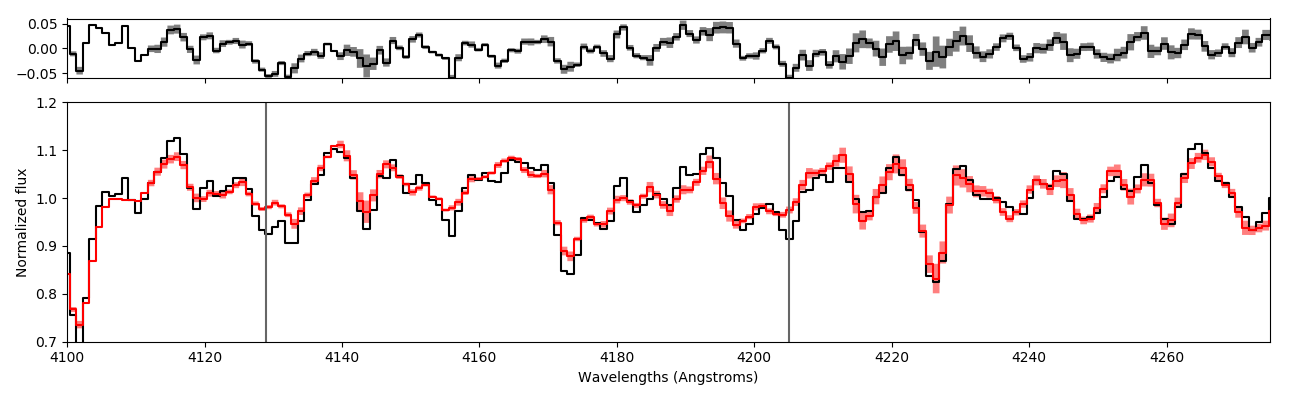
\includegraphics[width=\columnwidth]{423451}
		\caption{The spectral region around two Europium absorption lines at 4129 and 4205 Angstroms. This particular stars spectra (black) shows clear absorption at these wavelengths, as compared to the normalised spectra of a similar star (red).}
		\label{fig:starindex_423451}
	\end{figure}
	
	\begin{figure}
		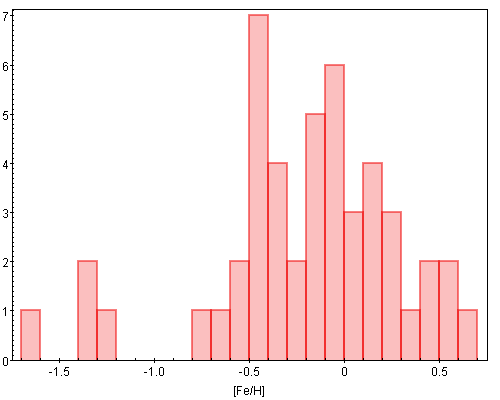
\includegraphics[width=\columnwidth]{NoTrend}
		\caption{The apparent lack of trends for the 47 enhanced stars. In three distinguishing categories: Metallicity (left), Effective Temperature (centre), and $log(g)$ (right).}
		\label{fig:starindex_423451}
	\end{figure}
	
	\section{Methods}
	
	\subsection{Observations and Candidate Selection}
	The LAMOST survey is a low resolution ($R\approx1800$) optical survey that took spectra of stars between (3650-9000 \AA). The LAMOST Data-Release 2 (DR2) collected spectra in this band for $\approx$ 2.2 million stars. Anna Ho describes in her 2017 paper (\cite{AnnaHo2017}) how she used a machine learning method named \textit{The Cannon}. \textit{The Cannon} fit a predictive model using 9952 LAMOST stars that were also found in the higher resolution ($R\approx22500$) APOGEE survey. \textit{The Cannon} was used to predict the labels $T_{eff}$, $log_{10}[g]$, $[Fe/H]$, and $[\alpha/Fe]$. From this Ho was able to fit normalised spectra to 454,180 giants from the LAMOST survey and was restricted to between 3905\,\AA\ and 9000\,\AA. For reference, typical uncertainties for these labels are $70K$ for $T_{eff}$, $0.1$ in $log_{10}[g]$, 0.1 in $[Fe/H]$, and 0.04 in $[\alpha/H]$.
	
	We selected potential candidate stars with an abundance of Europium by searching for deviations from the normalized spectra supplied by \textit{The Cannon}. A negative deviation implied an enhancement in a particular element while a positive deviation implied a depletion (compared to what the model expected). 
	
	At the two main absorption lines for Europium (4129\,\AA\ and 4205\,\AA) we fitted Gaussian profiles to each star in the 454,180 giants from LAMOST DR2, and we recorded the amplitude and the wavelength of each, as well as their corresponding errors. Candidate Eu-enhanced stars were identified by stars that met the following criteria:
	
	\begin{itemize}
		\item The amplitude of their deviation from the model needed to be less than -0.05 (remembering that a negative deviation corresponds to an enhancement in the element);
		\item The Signal to Noise (S/N) must have been greater than 30;
		\item The deviation from the required wavelength in question must have been less than 2 \AA;
		\item The $\chi^{2}$ value (where the $\chi^{2}$ value represents how well the rest of the model fit the spectrum, aside from the enhancement points) must have been less 3, and;
		\item All of these conditions must have been met for both 4129 and 4205 \AA for us to consider them sufficiently Eu enhanced.
	\end{itemize}   
	
	This left us with an initial sample of approximately 100 candidates out of the 454180 LAMOST giant sample. These were then visually scrutinised to find any that were clear outliers and did not belong in the sample. After this process we were left with 47 potentially r-process enhanced candidates, 22 of which stand out as very good candidates by comparison.
	
	\begin{figure}
		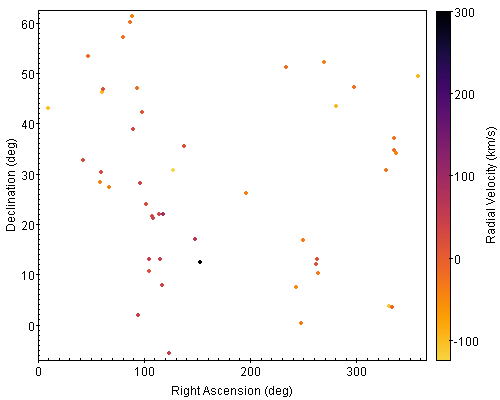
\includegraphics[width=\columnwidth]{RA_DEC_RadVel_48}
		\caption{The right ascension and declination for the enhanced stars, coloured by radial velocity. No clear trend or significant grouping is present.}
		\label{fig:radec_Eucands}
	\end{figure}
	
	\section{The r-process}
	For the r-process to occur there must be a very large neutron density, such that neutron capture must be able to occur before the nucleus undergoes a $\beta$-decay (assuming the nucleus is in an unstable state). The conditions that can create this are rare. Events such as supernovae or neutron star mergers list among the most favoured sites.
	
	\subsection{Selection effects}
	The LAMOST giants we analyse belong to a broad range of both metallicity and temperature, and don't cluster or trend towards any particular place in the observed sky. These characteristics and seeming lack-of a trend could argue that there must be multiple sites of the r-process. While rare events such as neutron star mergers may create r-process elements in a very high abundance in localised areas, it is improbable to assume that these rare events occur commonly enough across the observed sky to explain what we see here. We suggest instead that there exists another r-process site that is acting alongside neutron star mergers that is far more common, but produces far less r-process material, such as core-collapse supernovae.
	
	The previous sample of r-process stars, before the release of this letter, almost totally consists of metal-poor stars. This fact is not to be confused with saying that most r-process stars found should be metal-poor stars, rather that at low metallicities we know that the s-process will not contribute. So neutron capture elements formed from these stars would be only from the r-process. Similarly, over half the current known r-process stars come from a very metal poor ultra faint dwarf galaxy, Reticulum II. However, Europium we know to be almost totally made from the r-process, therefore even at metallicities where the s-process would be active, Europium is a valuable indication of r-process synthesis. 
	
	\subsection{Core-collapse supernovae}
	Core-collapse supernova was the site initially proposed to have a high enough neutron density in order to create elements synthesised by the r-process. The exact mechanism that leads to this high neutron density is so far unknown, but there have been promising theories and models in recent years that can explain r-process element synthesis in these conditions to an adequate degree. One of which is the action of high-entropy neutrino winds being released from a proto-neutron star during core-collapse. In this stage of the collapse, this neutrino loss is the driving factor behind mass loss and could be instrumental in the existence of the r-process in supernovae conditions. However how much enhanced material is released from the event is very dependant on the amount of material that falls back onto the remnant at the arrival of the reverse shock, and so often it may not release enough material to always be considered a site at which r-process material is expelled (\cite{Woosley1992}). Regardless of the exact mechanism, core-collapse supernovae seem to release $M_{Eu}\approx10^{-8}$ (\cite{Argast2004}) solar masses. While this may not be a particularly significant amount, core-collapse supernovae occur frequently in the Milky Way, and so it isn't unreasonable to suggest that much if not all r-process material could have been formed by these and recycled in the stars we present in this letter.
	
	\subsection{Neutron star mergers}
	\label{NSmerg}
	Neutron star mergers are another favoured possible site of r-process element synthesis, possibly the most favoured at the moment. They are easily able to meet the conditions for a high neutron density as interacting tidal forces between the stars rip away neutron dense material allowing r-process element synthesis to occur easily. In this interaction they produce a considerable amount more enriched material than core-collapse supernovae ($M_{Eu}\approx10^{-4.5}$) (\cite{Goriely2011}), however the direct interaction and merger of a binary neutron star pair occurs very infrequently with only one ever having been directly observed, and with an upper frequency estimate of $12600\ Gpc^{-3}yr^{-1}$ (\cite{LIGO2016}). The massive amount of material that these mergers release could more than make up for the low frequency and so, similar to core-collapse supernovae, it is not unreasonable to suggest that they are responsible for most if not all known r-process material. 

	The recent discovery of the UFD Reticulum II (\cite{Ji2016}) is evidence against the case for a single r-process site. Of nine stars observed in Reticulum II, 7 of them were shown to be highly enriched in r-process elements ([Eu/Fe]~1.7) which suggests a single prolific event having occurred in close proximity to the galaxy early in it's formation, such as a neutron star merger. However, two of the stars observed were only weakly enhanced in r-process elements which suggests that there must have been a second, less efficient, form of r-process enhancement present.
	
	\subsection{The rate of neutron star mergers, what we expect, what we find}
	From the recent aLIGO data \cite{LIGO2016}, we are able to find an estimate for an upper-bound frequency at which neutron star mergers occur, as mentioned in section \ref{NSmerg}. 
	Using this we are able to find:
	\begin{itemize}
		\item An estimate for the amount of r-process stars that should be present in the Milky Way that have been enhanced through neutron star mergers. Assuming instant recycling in that any star that dies is instantly formed into a new star, also assuming that no r-process matter pollutes other stars by any other means than this. 
		\item An estimate of how many r-process enhanced giants should be present from an estimate number of the Milky Way's total stars.
		\item An estimate of how many r-process enhanced stars (giants or otherwise) that should be present from an estimate number of the Milky Way's total stars.
	\end{itemize}
	
	In preparing these calculations we assumed a constant star formation rate, 2 M$_\odot yr^{-1}$, in the disk of the Milky Way, r=15kpc, with a typical IMF and giant star birth rate of approximately $0.3\ $stars per year. We also assumed the lifetime between $\log{g} = 3.2$ and the end of the core-helium burning phase is about $250\,{\rm Myr}$. Therefore if we assume a steady-state system, the number of giant stars in the Milky Way comes to approximately $7.53\times10^7$. This allowed us to find the percentage of the Milky Ways stars that our sample represents. \todo{I tried to make this explanation a fair bit different, let me know if it needs further changes.}
	
	In these calculations we also say that a star is said to be enhanced if [Eu/Fe] $\geq$ 0.7, and performed the low-bound estimate that all of our 47 stars exhibited this abundance. Additionally the amount of r-process material expelled is the same as previously discussed, using Europium as our identifier, of $M_{Eu}\approx10^{-4.5}$.
	
    We found from this that in the Milky Way alone there should be present 125589 r-process enhanced stars. Considering this should be considered a lower-bound estimate (by using the maximum rate for neutron star mergers, and assuming the lower bound Europium abundance) this is a startlingly large difference from the now updated known amount of r-process enhanced stars which comes to 60. 
    
    We also find that, of our sample of $\approx450000$ giants, the amount of r-process enhanced stars we should find comes to less than one (0.224). Similarly if we are to extend our sample from the 450000 giants supplied by Anna Ho, and instead use the entire LAMOST data release 2 (a survey of $\approx2.2$ million stars), we predict that we should have found 1.09 stars enhanced in the r-process. While again this should be considered a lower bound, it is still a startling difference from the 47 that we found in our sample.
    
    From these estimates we can also find an approximation for whether or not neutron star mergers by themselves are sufficient to enrich our entire r-process enhanced catalogue. We find that, by using the assumptions listed, neutron star mergers could create enough r-process material to enrich above the point of [Eu/Fe] > 0.7 for all 60 known r-process enhanced stars within $1.1\times10^9$ years. 
    
    
	%From Andy's Lithium paper.
%	I star formation rate of $2\,M_\odot\,{\rm yr}^{-1}$ and a typical initial mass function\cite{Kroupa_2001} and find a birth rate of giant stars in the Milky Way (the main-sequence turn-off rate) of about $0.3\,{\rm stars}\,{\rm yr}^{-1}$. 
%	We considered stellar masses between $0.1\,M_\odot$ and $100\,M_\odot$ when weighting the initial mass function.
%	For an evolutionary track \cite{MIST_Dotter,MIST_Choi} of a $1.3\,M_\odot$ solar-metallicity star, the lifetime between $\log{g} = 3.2$ and the end of the core-helium burning phase is about $250\,{\rm Myr}$. Thus, assuming a steady-state system, the number of giant stars in the Milky Way with $\log{g} < 3.2$ is about $7.5\times10^7$.
	
	\subsection{Multiple r-process sites?}
	While we've shown that all r-process material that we currently know of can be made by neutron star mergers, we still have cases of stars in the galaxy which show particularly weak enrichment from r-process elements ([Eu/Fe] < 0.7). While these enhancements are small, they are still very important as it implies that another site of r-process element synthesis is likely to be active. The neutron star merger rates may show that all heavily enriched stars can be enhanced by these phenomena within an adequate timescale, but we are not able to assume that as a consequence of the merger some stars are greatly enhanced, while others are only very slightly enhanced. Therefore it is better to assume that at least two sites exist, with one (potentially mergers) producing a massive abundance of enhanced material, and the other only producing some small amount, such as supernovae.
	
	\section{Conclusions}
	We present the largest to date sample of r-process element enhanced stars. These stars are found at a wide range of metallicities, contrary to previous discovery of only metal-poor r-process enhanced stars. Similarly they seem to show no trend in either temperatures, $log(g)$, or radial velocity. They don't cluster to any one end of the H-R diagram, so it is likely there is no correlation between type of star. They are found both in the disk and halo, and are not clustered anywhere in the sky. In addition to this we also present the first ever quantitative analysis, from information provided by aLIGO, that neutron star mergers possess the ability to synthesise all currently known r-process material in a feasible timescale. 
	
	We recommend follow-up high resolution spectra be obtained for each of the 47 stars to ascertain how enhanced they are. To find the origin of these stars and to show whether or not they may come from a similar progenitor site it is necessary to find orbits for them. We encourage orbit analysis after further Gaia data releases should these stars be present in them.
	
	\section*{Acknowledgements}
	
	We acknowledge Andrew Casey for reminding us of the volume of a sphere. Further acknowledgements are awarded to him for firing me less than the other two, so far.
	
	
	% The best way to enter references is to use BibTeX:
	
	\bibliographystyle{mnras}
	\bibliography{paper} % if your bibtex file is called example.bib
	\begin{thebibliography}{99}
		\bibitem[\protect\citeauthoryear{Sneden, C. et al.}{2008}]{Sneden2008}
		Sneden C., Cowan J.J., \& Gallino R. 2013, Annual review of Astronomy \& Astrophysics, 46, 1
		\bibitem[\protect\citeauthoryear{Ji, A. P. et al.}{2016}]{Ji2016}
		Ji A. P., Frebel A., Chiti A., \& Simon J. D. 2016, Nature, 531
		\bibitem[\protect\citeauthoryear{Ho et al.}{2017}]{AnnaHo2017}
		Ho A. Y. Q., Ness M. K., Hogg David W., Rix H-W., Liu C., Yang F., Zhang Y., Hou Y.,\& Wang Y. 2017, ApJ, 836, 1
		\bibitem[\protect\citeauthoryear{Burbidge, E. et al.}{1957}]{Burbidge1957}
		Burbidge E. M., Burbidge G. R., Fowler W. A., \& Hoyle F. 1957, Review of Modern Physics, 29, 4
		\bibitem[\protect\citeauthoryear{Goriely, S. et al.}{2011}]{Goriely2011}
		Goriely S., Bauswein A. \& Janka H-T. 2011, ApJ, 738, L32
		\bibitem[\protect\citeauthoryear{Abbott, B.P. et al.}{2016}]{LIGO2016}
		Abbot B.P. et al. 2011, ApJ, 832, L21
		\bibitem[\protect\citeauthoryear{Argast, D. et al.}{2004}]{Argast2004}
		Argast D., Samland M., Thielmann F-K. \& Qian Y-Z. 2004, Astronomy and Astrophysics, 416
		\bibitem[\protect\citeauthoryear{Woosley, S.E. et al.}{1992}]{Woosley1992}
		Woosley S.E, \& Hoffman R.D. 1992, ApJ, 395, 1
	\end{thebibliography}
	
	
	
	\appendix
	\section{Some extra material}
	
	If you want to present additional material which would interrupt the flow of the main paper,
	it can be placed in an Appendix which appears after the list of references.
	
	\begin{table*}
		\centering
		\resizebox{\textwidth}{!}{%
			\begin{tabular}{@{}llllllllllllll@{}}
				\toprule
				\textbf{2MASS ID} & \textbf{RA} & \textbf{DEC} & \textbf{S/N} & \textbf{\begin{tabular}[c]{@{}l@{}}Vr\\ (km/s)\end{tabular}} & \textbf{Teff} & \textbf{Logg} & \textbf{{[}Fe/H{]}} & \textbf{{[}$\alpha$/Fe{]}} & \textbf{$\chi^{2}$} & \textbf{\begin{tabular}[c]{@{}l@{}}{[}Eu/Fe{]}\\ at 4129\end{tabular}} & \textbf{\begin{tabular}[c]{@{}l@{}}{[}Eu/Fe{]}\\ at 4129 error\end{tabular}} & \textbf{\begin{tabular}[c]{@{}l@{}}{[}Eu/Fe{]}\\ at 4205\end{tabular}} & \textbf{\begin{tabular}[c]{@{}l@{}}{[}Eu/Fe{]}\\ at 4205 error\end{tabular}} \\ \midrule
				J063400.95+420904.3 & 34:01.0 & +42:09:04.4 & 34.09 & 9.89 & 4315.56 & 1.62 & -0.50 & 0.10 & 0.43 & 1.02 & 3.09 & 1.35 & 0.22 \\ \midrule
				J220118.66+033558.6 & 01:18.7 & +03:35:58.6 & 35.11 & -108.23 & 4790.06 & 2.51 & -1.36 & 0.33 & 0.37 & 1.51 & 0.03 & 1.38 & 0.16 \\ \midrule
				J060021.29+384840.6 & 00:21.3 & +38:48:40.6 & 30.03 & 32.68 & 4305.08 & 2.10 & 0.15 & -0.01 & 0.54 & 1.48 & 0.29 & 1.51 & 0.04 \\ \midrule
				J025225.88+324308.1 & 52:25.9 & +32:43:08.2 & 34.79 & 24.88 & 4797.58 & 2.52 & -0.23 & 0.05 & 0.24 & 1.32 & 0.16 & 1.31 & 0.14 \\ \midrule
				J163116.81+002349.5 & 31:16.8 & +00:23:49.5 & 32.63 & -35.98 & 4628.92 & 2.53 & 0.01 & 0.18 & 0.29 & 1.37 & 0.25 & 1.51 & 0.03 \\ \midrule
				J153333.12+510621.8 & 33:33.1 & +51:06:21.9 & 49.45 & -17.99 & 4861.78 & 2.51 & -0.49 & 0.22 & 0.46 & 1.33 & 0.16 & 1.29 & 0.12 \\ \midrule
				J075116.55+220137.8 & 51:16.6 & +22:01:37.9 & 32.87 & 90.24 & 4810.60 & 2.70 & -0.33 & 0.02 & 0.30 & 1.38 & 0.18 & 1.32 & 0.15 \\ \midrule
				J003929.43+430039.5 & 39:29.4 & +43:00:39.6 & 33.14 & -104.33 & 4190.26 & 1.87 & -0.01 & 0.07 & 0.41 & 1.37 & 0.19 & 1.33 & 0.19 \\ \midrule
				J071206.83+213038.0 & 12:06.8 & +21:30:38.1 & 32.66 & 29.08 & 4432.03 & 1.75 & -0.38 & 0.11 & 0.40 & 1.51 & 0.03 & 1.43 & 0.19 \\ \midrule
				J222820.22+340750.3 & 28:20.2 & +34:07:50.3 & 34.52 & -45.27 & 4419.96 & 2.06 & -0.07 & 0.11 & 0.49 & 1.36 & 0.17 & 1.38 & 0.17 \\ \midrule
				J222310.49+344357.4 & 23:10.5 & +34:43:57.5 & 54.06 & -20.09 & 4232.66 & 1.87 & -0.01 & 0.03 & 0.86 & 1.27 & 0.09 & 1.18 & 0.21 \\ \midrule
				J222101.61+365923.6 & 21:01.6 & +36:59:23.7 & 30.81 & -27.88 & 4360.28 & 2.23 & 0.20 & 0.04 & 0.45 & 1.51 & 0.03 & 1.42 & 0.21 \\ \midrule
				J074102.63+130520.3 & 41:02.6 & +13:05:20.4 & 40.83 & 49.17 & 5000.84 & 3.00 & -0.38 & -0.02 & 0.30 & 1.27 & 0.15 & 1.42 & 0.12 \\ \midrule
				J061559.10+470344.9 & 15:59.1 & +47:03:44.9 & 36.84 & -18.29 & 4811.98 & 2.82 & -0.59 & 0.07 & 0.44 & 0.63 & 1.30 & 1.37 & 0.13 \\ \midrule
				J054704.12+600827.1 & 47:04.1 & +60:08:27.1 & 33.19 & -23.33 & 4770.80 & 2.64 & -0.10 & 0.06 & 0.40 & 1.51 & 0.03 & 1.40 & 0.16 \\ \midrule
				J042723.73+271546.8 & 27:23.7 & +27:15:46.9 & 45.73 & -40.17 & 4211.91 & 1.72 & -0.04 & 0.05 & 0.79 & 1.36 & 0.20 & 1.30 & 0.18 \\ \midrule
				J035702.05+281335.2 & 57:02.1 & +28:13:35.3 & 31.82 & -44.67 & 4712.89 & 2.44 & 0.01 & 0.16 & 0.46 & 1.35 & 0.14 & 1.22 & 0.29 \\ \midrule
				J091256.32+353008.3 & 12:56.3 & +35:30:08.3 & 73.39 & 20.39 & 4441.95 & 2.33 & 0.41 & 0.02 & 0.76 & 0.61 & 0.30 & 1.24 & 0.14 \\ \midrule
				J071534.00+211353.8 & 15:34.0 & +21:13:53.9 & 31.68 & 42.27 & 4892.00 & 2.57 & -0.72 & 0.11 & 0.34 & -0.20 & 0.00 & 1.38 & 0.21 \\ \midrule
				J101317.14+122928.8 & 13:17.1 & +12:29:28.8 & 45.54 & 300.69 & 5055.95 & 2.24 & -1.34 & 0.33 & 0.38 & 1.51 & 0.03 & 1.41 & 0.14 \\ \midrule
				J161326.00+073218.1 & 13:26.0 & +07:32:18.2 & 48.45 & -50.07 & 5086.79 & 3.40 & -0.68 & 0.29 & 0.93 & 1.44 & 0.11 & 1.32 & 0.08 \\ \midrule
				J173711.85+101126.6 & 37:11.9 & +10:11:26.7 & 30.01 & -33.58 & 4991.07 & 3.49 & -0.05 & 0.17 & 0.41 & 1.40 & 0.15 & 1.50 & 0.13 \\ \bottomrule
			\end{tabular}%
		}
		\caption{Abundances and additional information of the comparatively very good candidates. Abundances were found from the LAMOST data.}
		\label{Eu for the great 22}
	\end{table*}
	
	% Don't change these lines
	%\bsp	% typesetting comment
	\label{lastpage}
\end{document}
